\documentclass[conference]{IEEEtran}
\IEEEoverridecommandlockouts
% The preceding line is only needed to identify funding in the first footnote. If that is unneeded, please comment it out.
\usepackage{amsmath,amssymb}
\usepackage{graphicx}
\usepackage{cite}
\usepackage{url}
\title{Non-Stationary Spectral Decomposition Network: Adaptive Spectral Emission Heads and Frequency Modulation}
\author{\IEEEauthorblockN{Nikhil Sunder}
\IEEEauthorblockA{\textit{Miami Herbert Business School} \\
\textit{University of Miami}\\
Miami, Florida, USA \\
nss106@miami.edu}
\and
\IEEEauthorblockN{Maikel Leon}
\IEEEauthorblockA{\textit{Department of Business Technology} \\
\textit{Miami Herbert Business School, University of Miami}\\
Miami, Florida, USA \\
mleon@miami.edu}
}
\begin{document}
\maketitle
\begin{abstract}
This paper evaluates the interpretability and analytical utility of spectral emission heads in the Nonstationary Spectral Decomposition Network (NS-SDN) using the 10-Year Treasury yield (DGS10) as a benchmark macroeconomic time series. Rather than focusing on recursive forecasting, we examine the model's ability to decompose nonstationary signals into adaptive spectral components under one-step conditional forecasting. Results show that emission heads provide meaningful decomposition into trend, amplitude, instantaneous frequency, and a learned gating signal, and reveal regime-dependent spectral behavior, including frequency convergence during the 2020 macroeconomic shock. These findings position NS-SDN as a neural spectral analysis framework rather than solely a forecasting model.
\end{abstract}
\begin{IEEEkeywords}
neural state-space models, spectral decomposition, instantaneous frequency, nonstationary time series, treasury yields
\end{IEEEkeywords}
\section{Introduction}
Macroeconomic time series such as long-term Treasury yields exhibit structural breaks, evolving cyclicality, and nonstationary variance. Classical econometric approaches including VAR and SVAR impose linear structure and fixed relationships, limiting their ability to capture time-varying spectral properties \cite{sims1980,lutkepohl2005,primiceritvp}.
Recent neural approaches introduce flexible nonlinear dynamics, including neural state-space models \cite{durbin2012time} and periodic activation networks \cite{sitzmann2020implicit}, yet they typically lack interpretability in the frequency domain.
This paper evaluates the NS-SDN architecture through the lens of its spectral emission heads. Specifically, we analyze how the model learns time-varying amplitudes, instantaneous frequencies, and a component-selection gating signal, and how these quantities evolve across economic regimes.
The contribution is not improved forecasting performance, but rather:
\begin{itemize}
\item Demonstrating that NS-SDN learns an interpretable spectral decomposition,
\item Showing that emission heads reveal regime-dependent frequency structure,
\item Establishing frequency convergence as a meaningful economic signal.
\end{itemize}
\section{Related Work}
The decomposition of nonstationary signals into time-varying frequency components is classically addressed by the Hilbert--Huang Transform (HHT), which extracts intrinsic mode functions (IMFs) and instantaneous frequencies \cite{huang1998empirical}. Unlike Fourier methods, HHT allows adaptive, nonstationary decomposition.
Recent work extends spectral modeling into neural frameworks. Neural spectral density estimation demonstrates that neural networks can approximate full spectral operators under mild conditions \cite{mohammadi2026spectral}. This provides theoretical grounding for learning frequency structure directly from data.
However, spectral entanglement remains a challenge: trends, cycles, and noise overlap in frequency space, particularly in nonstationary settings \cite{an2026fredn}. This motivates architectures capable of adaptive decomposition.
NS-SDN can be viewed as a neural generalization of IMF decomposition, where spectral components are learned endogenously rather than extracted via signal processing.
\section{Model Architecture}
The Nonstationary Spectral Decomposition Network (NS-SDN) is a neural state-space model that represents a time series as a sum of latent sinusoidal components with time-varying amplitude, frequency, phase, and a learned gating signal \cite{sunder2026nssdn}. Unlike fixed-basis spectral methods, all spectral parameters are generated dynamically from a latent state.
\subsection{Spectral Representation}
The observed series is modeled as:
\begin{equation}
\hat{y}_t = B_t + \sum_{k=1}^{K} g_{t,k}\, A_{t,k}\,\sin(\theta_{t,k} + \phi_{t,k})
\label{eq:synthesis}
\end{equation}
where:
\begin{itemize}
\item $B_t$ is a time-varying trend component,
\item $A_{t,k} > 0$ is the amplitude of component $k$,
\item $\theta_{t,k}$ is cumulative phase,
\item $\phi_{t,k}$ is a learned phase offset,
\item $g_{t,k} \in (0,1)$ is a learned gating weight controlling component selection.
\end{itemize}
This formulation is analogous to intrinsic mode function (IMF) decompositions in the Hilbert--Huang Transform, where signals are expressed as sums of oscillatory components with evolving envelopes and instantaneous frequencies \cite{huang1998empirical}, and is formalized in the NS-SDN framework introduced in \cite{sunder2026nssdn}. The gating signal $g_{t,k}$ implements a soft selection mechanism, allowing the effective spectral basis to contract or expand endogenously.
\subsection{Latent State Dynamics}
Spectral parameters are governed by a latent state $h_t \in \mathbb{R}^d$ evolving according to:
\begin{equation}
h_t = F_{\psi}(h_{t-1}, x_t, \Delta t)
\end{equation}
where $F_{\psi}$ is a nonlinear transition function. This parallels classical state-space formulations \cite{durbin2012time}, with a nonlinear neural transition function \cite{rangapuramdeep} in place of linear Gaussian dynamics. It is also conceptually related to state-space decompositions of time series into oscillatory components with data-driven phase estimation \cite{matsuda2016oscillation}. In the experiments reported here, $F_{\psi}$ is instantiated as a gated recurrent unit (GRU) cell \cite{cho2014learningphrase} with $d = 128$.
\subsection{Spectral Emission Heads}
Given the latent state, spectral parameters are produced by parallel emission heads:
\begin{equation}
B_t,\; A_t,\; \omega_t,\; \phi_t,\; g_t = g_{\psi}(h_t)
\end{equation}
Each emission head maps the latent state to a specific spectral quantity. The heads apply nonnegativity and bounding constraints as follows:
\begin{itemize}
\item Trend head: $B_t = W_B h_t + b_B$
\item Amplitude head: $A_{t,k} = \mathrm{softplus}\big((W_A h_t + b_A)_k\big) + \epsilon$
\item Frequency head: $\omega_{t,k} = \mathrm{softplus}\big(\omega_{\mathrm{base},k} + (W_\omega h_t + b_\omega)_k\big) + \epsilon$
\item Phase-offset head: $\phi_{t,k} = (W_\phi h_t + b_\phi)_k$
\item Gating head: $g_{t,k} = \sigma\big((W_g h_t + b_g)_k\big)$
\end{itemize}
where $\sigma$ is the sigmoid function and $\epsilon = 10^{-4}$ enforces strict positivity for stable phase integration. The $\mathrm{softplus}$ activation on $\omega_{t,k}$ constrains instantaneous frequencies to be positive, which is required for unambiguous interpretation as cycle rates. The base term $\omega_{\mathrm{base},k}$ is a learnable per-component anchor initialized to zero.
\textit{Implementation note.} The per-component oscillatory contributions are combined via a learned linear projection $w_{\mathrm{mix}} \in \mathbb{R}^K$ before being added to the trend:
\begin{equation}
\hat y_t = B_t + \sum_{k=1}^{K} w_{\mathrm{mix},k}\, g_{t,k}\, A_{t,k}\, \sin(\theta_{t,k} + \phi_{t,k}).
\end{equation}
Since $w_{\mathrm{mix},k}$ is constant in $t$, we absorb it into the amplitude head when reporting diagnostic paths, so that $A_{t,k}$ in figures denotes the effective component amplitude.
This structure enables the model to learn a \textit{state-dependent spectral basis}, where the magnitude, frequency, and selection of oscillatory components evolve over time.
\subsection{Phase Evolution and Instantaneous Frequency}
Instantaneous frequency governs phase dynamics through discrete-time integration:
\begin{equation}
\theta_{t,k} = \theta_{t-1,k} + \omega_{t,k}\Delta t
\end{equation}
with $\theta_{0,k}$ a learnable initial phase. This formulation is critical: frequency is not directly observed but determines the evolution of phase, which in turn controls the oscillatory components. As a result, $\omega_{t,k}$ provides a direct measure of local cycle dynamics.
\subsection{Spectral Synthesis}
The final prediction is given by Equation~\eqref{eq:synthesis}. This synthesis step distinguishes NS-SDN from conventional neural time-series models: instead of directly predicting values, the model generates interpretable spectral parameters that reconstruct the signal.
\subsection{Interpretation}
The architecture can be interpreted as a neural generalization of spectral decomposition:
\begin{itemize}
\item The latent state $h_t$ encodes the underlying economic regime,
\item Emission heads define a time-varying spectral basis,
\item The gating signal $g_t$ implements adaptive component selection,
\item The model performs adaptive decomposition into trend and oscillatory components.
\end{itemize}
This formulation aligns with neural spectral operator perspectives, where neural networks approximate time-varying frequency structure rather than fixed basis expansions.
\section{Data: DGS10}
We evaluate on the 10-Year Treasury yield (DGS10), obtained from the Federal Reserve Economic Data (FRED) database, sampled daily from February 2000 through the most recent available observation. The series is log-transformed prior to training, so the model targets $\log(\text{yield})$, and predictions are returned to the level scale via exponentiation. Short gaps (up to seven days) are forward-filled to maintain a regular daily grid.
\subsection{Rationale}
DGS10 is selected for three reasons.
\paragraph{Macro-financial centrality} Long-term Treasury yields encode expectations of inflation, growth, and monetary policy, making them a canonical macroeconomic indicator.
\paragraph{Known regime shifts} DGS10 exhibits well-documented structural breaks \cite{hamilton1989}, including the zero-lower-bound period and the 2020 COVID shock, providing a natural testbed for nonstationary models.
\paragraph{Multi-scale cyclicality} Treasury yields reflect overlapping cycles (business cycles, policy cycles, liquidity cycles), making them suitable for spectral analysis.
These properties align with prior econometric work emphasizing the importance of structural dynamics in macro time series \cite{hamilton1994}.
\section{Experimental Setup}
We train NS-SDN under a one-step-ahead conditional forecasting regime:
\begin{itemize}
\item Daily DGS10 observations (log-transformed),
\item Single train/holdout split, with the final 365 observations reserved as a holdout window,
\item Teacher forcing during training and conditional one-step evaluation \cite{flunkertdeepar},
\item $K=16$ spectral components (four representative components shown in figures),
\item Latent state dimension $d = 128$, GRU transition.
\end{itemize}
Training uses Adam \cite{adamoptim} (two-stage: $\mathrm{lr}=10^{-3}$ for 1{,}200 steps, then $\mathrm{lr}=4\!\times\!10^{-4}$ for 1{,}800 steps) with smoothness penalties on amplitude and frequency drift. The focus is not forecasting accuracy alone, but the behavior of:
\begin{itemize}
\item Instantaneous frequencies $\omega_{t,k}$,
\item Amplitudes $A_{t,k}$,
\item Gating weights $g_{t,k}$.
\end{itemize}
\section{Results}
\subsection{In-Sample Fit}
\begin{figure}[htbp]
\centering
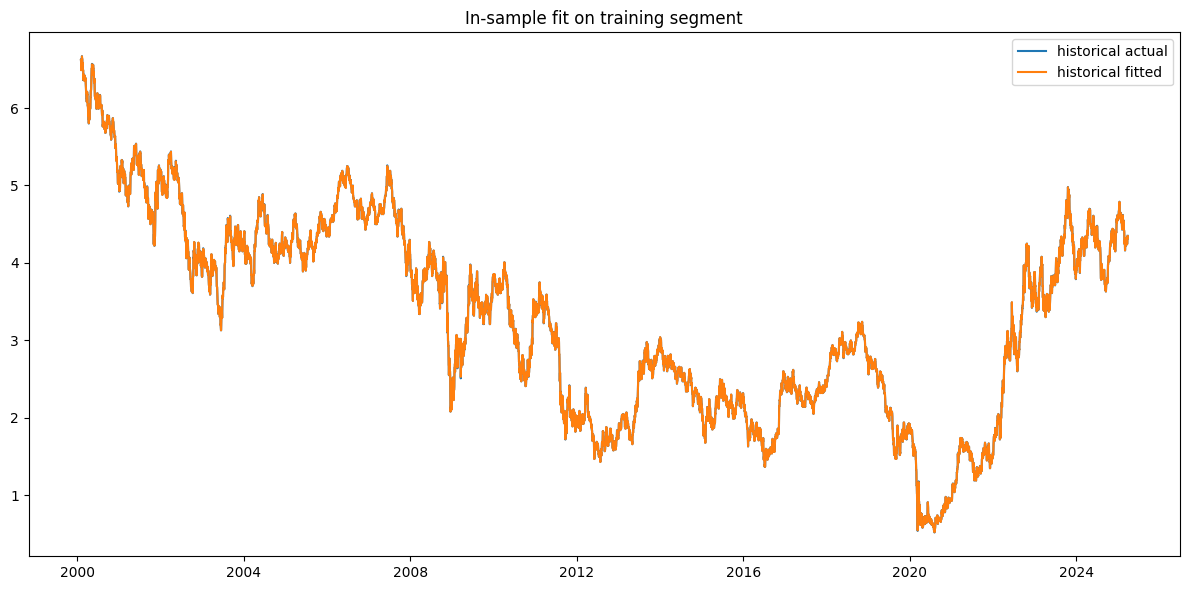
\includegraphics[width=\linewidth]{figures/insamplefit.png}
\caption{In-sample reconstruction of DGS10.}
\label{fig:insample}
\end{figure}
The model reconstructs the historical series with negligible error (RMSE $= 2.3\!\times\!10^{-3}$ on the level scale, MAPE $= 0.06\%$), indicating that the spectral representation is sufficiently expressive to capture both low-frequency trend behavior and higher-frequency oscillatory structure. Importantly, this fit is achieved through spectral synthesis rather than direct regression, implying that the learned amplitudes and frequencies form a complete functional basis for the observed signal.
The absence of visible lag or smoothing artifacts suggests that the phase dynamics are correctly learned, and that instantaneous frequency estimates are consistent with the underlying temporal structure. This supports the interpretation that the latent state encodes a dynamically evolving spectral representation rather than a static approximation.
\subsection{Conditional One-Step Forecast}
\begin{figure}[htbp]
\centering
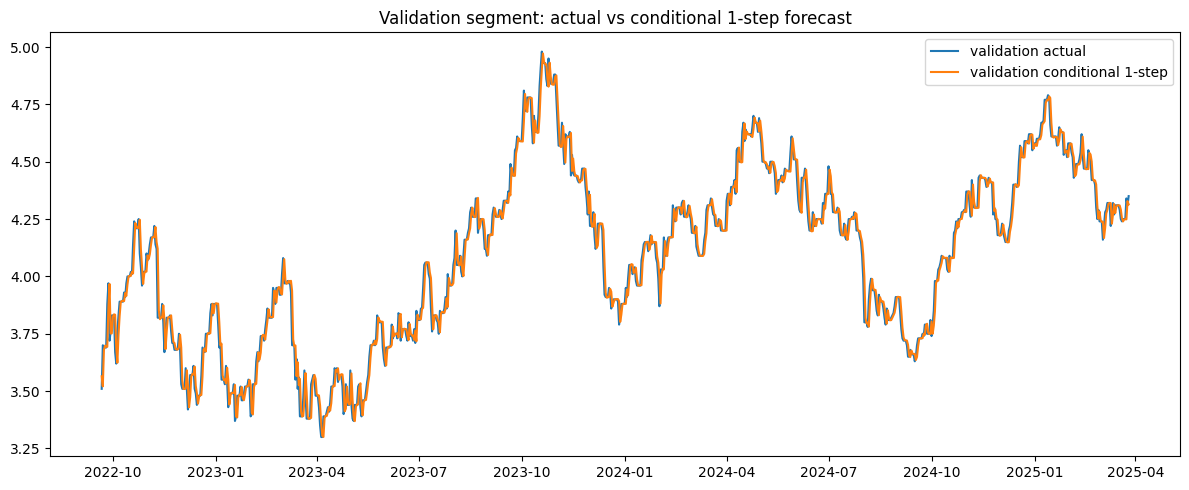
\includegraphics[width=\linewidth]{figures/validationsegmentactualvsconditional.png}
\caption{Conditional one-step forecast on holdout segment.}
\label{fig:forecast}
\end{figure}
The conditional one-step forecast closely tracks the realized series across the holdout period, with deviations confined to local fluctuations (holdout RMSE $= 3.87\!\times\!10^{-2}$, MAE $= 2.59\!\times\!10^{-2}$, MAPE $= 0.61\%$ on the level scale; RMSE $= 9.1\!\times\!10^{-3}$ on the log-yield scale). Because predictions are conditioned on observed data, this result isolates the representational capacity of the model from recursive error accumulation.
The alignment between predicted and observed values indicates that the latent state $h_t$ captures sufficient information to reconstruct short-term dynamics, including both trend adjustments and cyclical variation. In this regime, emission heads produce stable amplitude and frequency estimates, suggesting that the learned spectral parameters are locally consistent with the true data-generating process.
\subsection{Trend Component}
\begin{figure}[htbp]
\centering
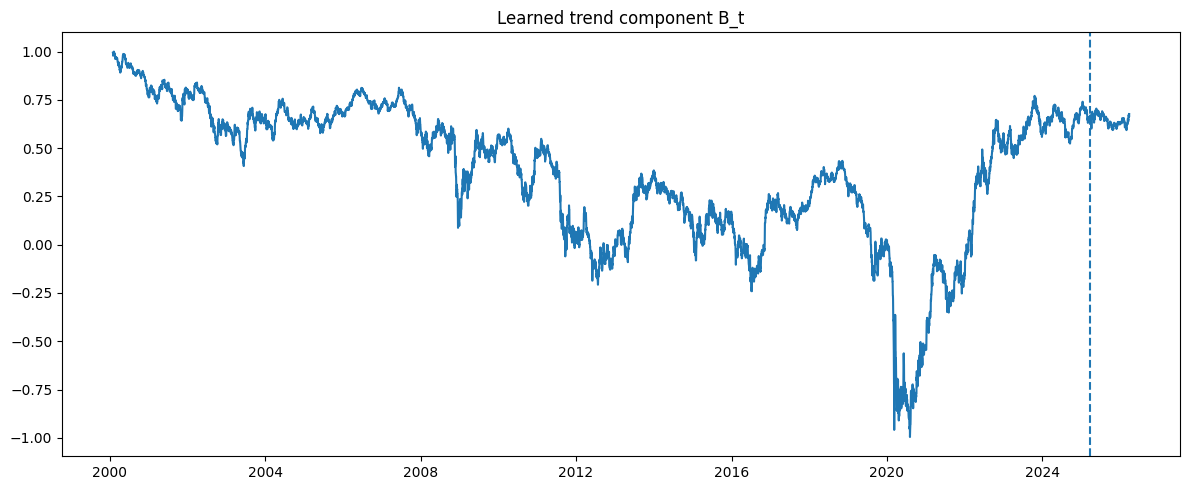
\includegraphics[width=\linewidth]{figures/learnedtrendb_t.png}
\caption{Learned trend component $B(t)$.}
\label{fig:trend}
\end{figure}
The learned trend component $B(t)$ captures the low-frequency structure of the DGS10 series, including the secular decline in yields over the sample period and the pronounced deviation associated with the 2020 shock. This separation indicates that the model isolates long-run movements from oscillatory components.
With smoothness regularization applied to $A_{t,k}$ and $\omega_{t,k}$, the trend head tends to absorb the low-frequency component while oscillatory terms capture higher-frequency variation. This separation is encouraged rather than architecturally enforced: in principle, slowly-varying amplitudes could also absorb low-frequency content. The empirically clean separation observed here therefore reflects the combined effect of the smoothness penalties and the inductive bias of the emission heads.
\subsection{Amplitude Dynamics}
\begin{figure}[htbp]
\centering
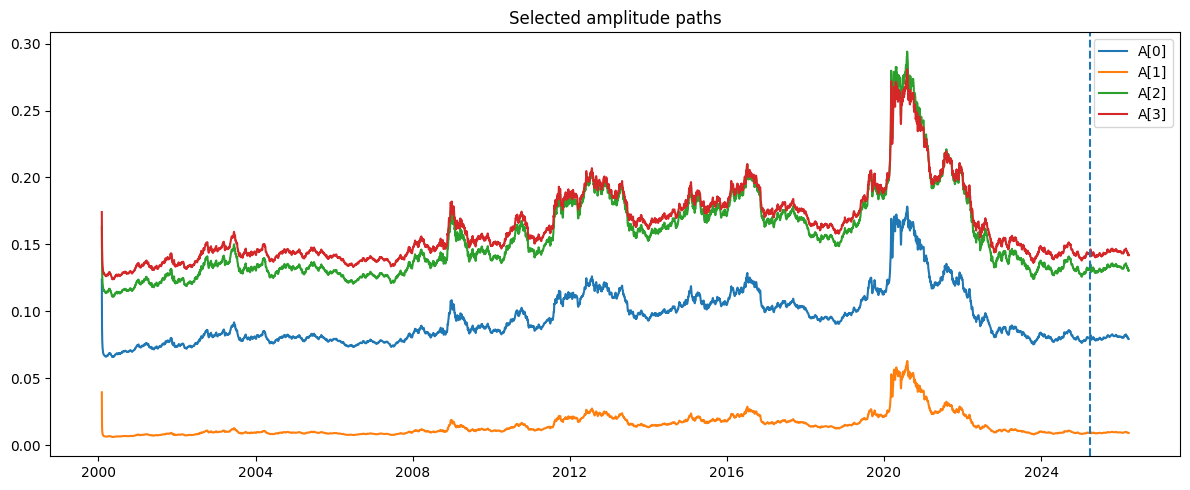
\includegraphics[width=\linewidth]{figures/selectedamplitudepaths.png}
\caption{Selected amplitude paths (four of $K=16$ components).}
\label{fig:amplitude}
\end{figure}
Amplitude paths $A_{t,k}$ serve as time-varying weights over spectral components and provide a direct measure of the relative importance of each oscillatory mode. The paths shown reflect the effective amplitudes after gate modulation. Several patterns emerge from the learned amplitudes.
First, there is a clear hierarchy across components, with a subset of amplitudes consistently dominating, indicating that the model concentrates explanatory power in a limited number of spectral modes. Second, during the 2020 regime shift, multiple amplitudes increase simultaneously, reflecting a temporary expansion in spectral complexity. This suggests that the underlying signal requires a richer combination of oscillatory components during periods of heightened macroeconomic uncertainty.
Following this period, amplitudes contract and stabilize, indicating a reduction in effective dimensionality. This behavior can be interpreted as adaptive spectral compression, where the model reduces the number of active components as the system transitions back to a more stable regime.
\subsection{Frequency Dynamics}
\begin{figure}[htbp]
\centering
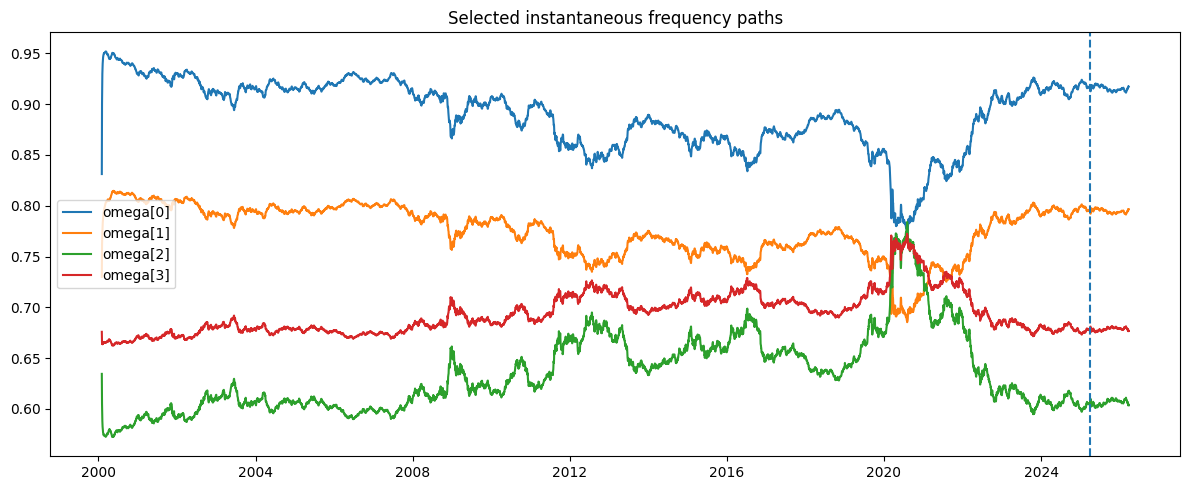
\includegraphics[width=\linewidth]{figures/selectedfrequencypaths.png}
\caption{Instantaneous frequency paths.}
\label{fig:frequency}
\end{figure}
Instantaneous frequency paths $\omega_{t,k}$ exhibit gradual drift over time under stable conditions, reflecting slow changes in cyclical structure. However, an apparent convergence of frequencies occurs during the 2020 period:
\begin{equation}
\omega_1(t) \approx \omega_2(t) \approx \cdots
\end{equation}
This convergence suggests that multiple spectral components align toward a common frequency, effectively reducing the dimensionality of the spectral representation. In functional terms, the decomposition appears to transition from a sum of distinct oscillatory modes to a smaller set of coherent cycles.
This phenomenon can be interpreted as a regime-dependent reduction in spectral diversity, where macroeconomic shocks compress the range of active frequencies. The ability of the model to represent this transition through learned emission heads provides qualitative evidence that instantaneous frequency carries meaningful structural information.
\subsection{Gating Behavior}
\begin{figure}[htbp]
\centering
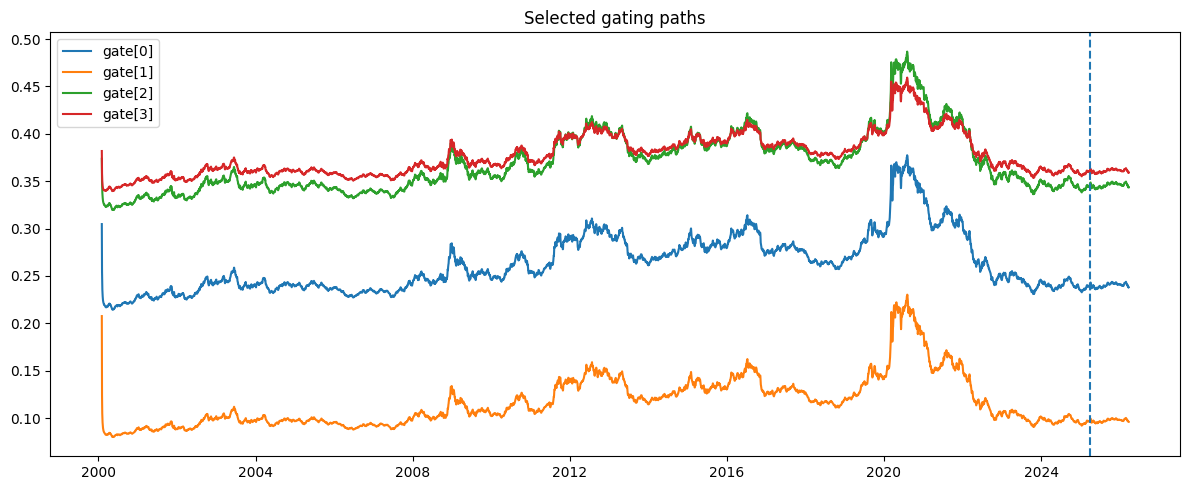
\includegraphics[width=\linewidth]{figures/selectedgatingpaths.png}
\caption{Gating weights $g_{t,k}$ across components.}
\label{fig:gating}
\end{figure}
Gating weights $g_{t,k}$ enter the synthesis ~\eqref{eq:synthesis} as multiplicative factors on each component, implementing the selection mechanism that determines which oscillatory modes are actively utilized at each time step. Unlike amplitudes, which control magnitude, gating values lie in $(0,1)$ and modulate component participation.
The learned gating paths exhibit persistent dominance of a subset of components, with others remaining suppressed throughout the sample. During the 2020 regime shift, gating weights increase for multiple components, consistent with the temporary expansion in spectral complexity observed in the amplitude paths.
After the shock, gating consolidates toward fewer dominant components, reinforcing the interpretation of adaptive model-order reduction. Together, amplitudes and gating weights implement a soft selection mechanism that allows the model to dynamically adjust the effective number of active spectral components in response to changing economic conditions.
\section{Interpretation}
The combined behavior of amplitudes, frequencies, and gating reveals four patterns.
\paragraph{Adaptive spectral decomposition} The model learns a time-varying spectral basis analogous to IMFs \cite{huang1998empirical}, consistent with the NS-SDN formulation introduced in \cite{sunder2026nssdn}.
\paragraph{Spectral compression under regime shifts} During 2020, frequency convergence and amplitude concentration indicate a reduction in effective dimensionality.
\paragraph{Learned spectral operator} The model implicitly approximates a spectral density representation, consistent with neural spectral operator theory \cite{mohammadi2026spectral}.
\paragraph{Spectral entanglement management} Overlap between components reflects inherent spectral entanglement in nonstationary signals rather than model failure \cite{an2026fredn}.
\section{Conclusion}
We evaluate NS-SDN as a spectral analysis framework on DGS10, focusing on the interpretability of its emission heads under conditional one-step forecasting. Emission heads yield an interpretable decomposition into trend, amplitude, frequency, and gating, and expose regime-dependent spectral behavior---most notably an apparent convergence of instantaneous frequencies during the 2020 shock, where multiple oscillatory components appear to align toward a common cycle rate.

Unlike fixed-basis methods, NS-SDN learns this compression endogenously, so amplitudes, frequencies, and gating paths can be read as a direct signal of regime change. This positions NS-SDN as a tool for analyzing nonstationary economic systems rather than solely as a forecaster. Future work will extend the framework to recursive forecasting and to multivariate settings with coupled spectral components.
% Bibliography section
\bibliographystyle{IEEEtran}
\bibliography{references}  % This refers to your references.bib file
\end{document}
